\chapter{Addestramento rete neurale}\label{addestramento-rete-neurale}


Come già menzionato nei capitoli precedenti l’idea è quella di allenare una \gls{cnn} per la classificazione dei frame di una laringoscopia attraverso il transfer learning. Utilizzando la tecnica del
fine-tuning nelle due varianti (One Round Tuning e Two Round Tuning)  su una rete pre-allenata chiamata AlexNet.


Viene usato un addestramento \(k\)-fold, in particolare con \(k=3\), in ogni fold i  pattern vengono elaborati con un
ordine diverso e si utilizza circa il 2/3 di essi come test set.


\section{Allenamento 1R}\label{allenamento-1r}

La sperimentazione inizia con l'allenamento della \gls{cnn} con un fine-tuning standard e classico (denominato anche One Round Tuning, descritto in \cref{one-round-tuning}), nel senso che si rimpiazzano gli ultimi 3 layer e poi si riallena la rete. Come dataset è stato usato il dataset descritto NBI-InfFrames in \cref{descrizione-dei-dataset}. È da prestare attenzione ai vari iperparametri, come \Gls{LearningRate} e \Gls{MiniBatchSize}. In particolare, è stato usato un learning rate di 0.0001 e un mini batch size di 30, il metodo di ottimizzazione è lo \gls{sgd}. Come data augmentation sono stati usati i valori descritti nel \cref{data-augmentation}, in questo caso non è stata usata la discrete cousene transform. La confusion matrix di questo allenamento è mostrato in \cref{fig:result-one-liscio}.


\begin{figure}[H]
    \centering
    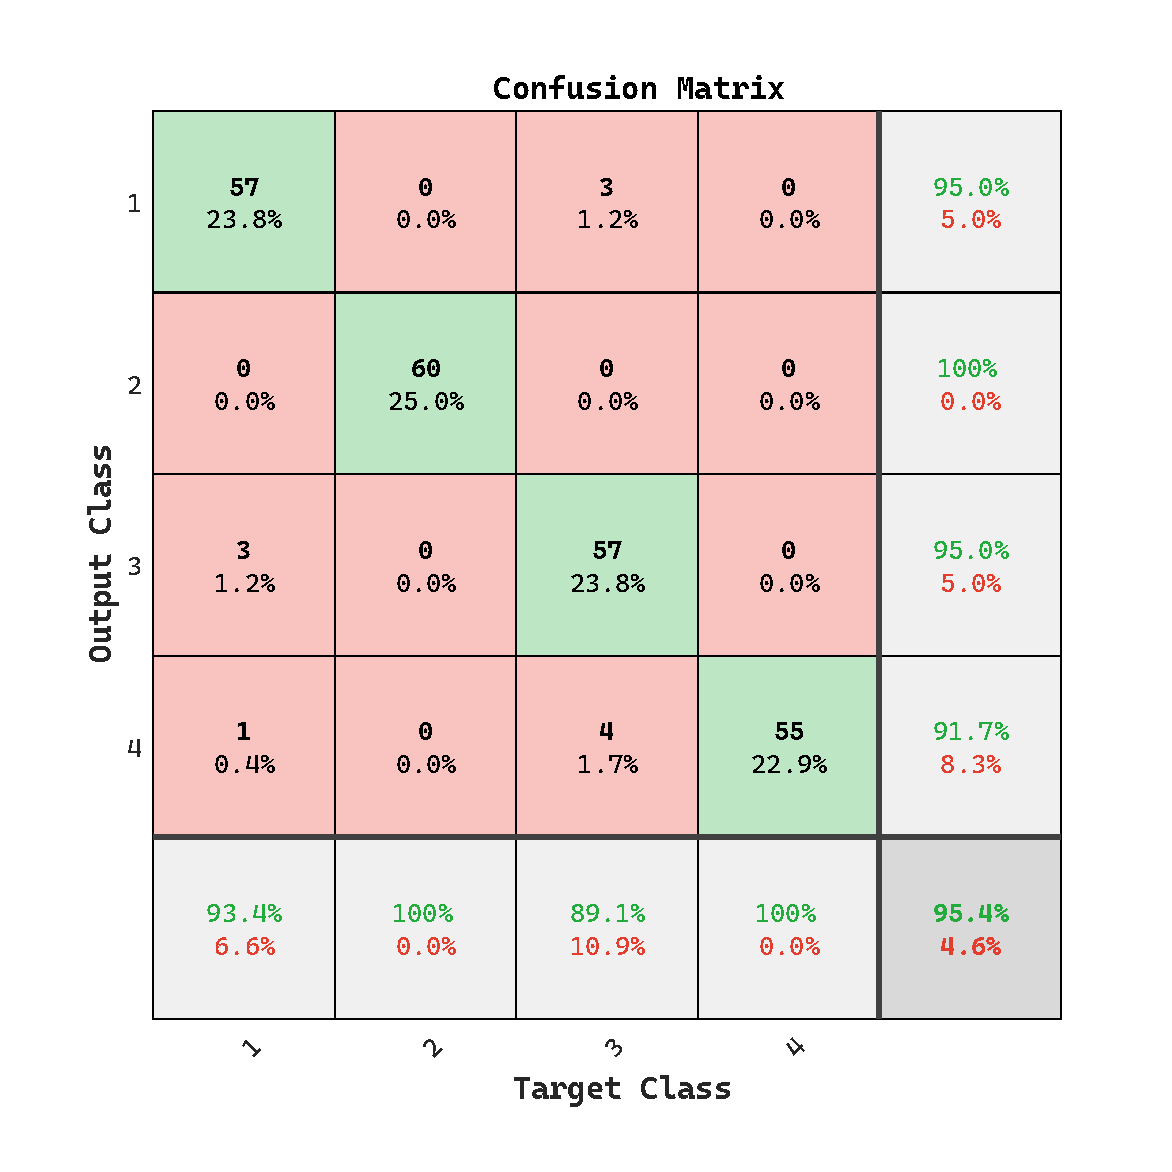
\includegraphics[width=0.49\textwidth]{addestramento-rete-neurale/one-liscio.pdf}
    \caption{Confusion matrix dell'allenamento con TL 1R senza preprocessing e con una semplice data augmentation}
    \label{fig:result-one-liscio}
\end{figure}

\section{Allenamento 2R}\label{allenamento-2r}

L'allenamento 2R descritto in \cref{two-round-tuning} è composto da una prima fase di allenamento con un dataset similare e poi il dataset NBI-InfFrames, entrambi descritti in  \cref{descrizione-dei-dataset}. In questo caso gli iperparametri sono:   learning rate di 0.0001 e un mini batch size di 30, il metodo di ottimizzazione è il \gls{sgd}, come data argumentation sono stati usati i valori descritti nel \cref{data-augmentation} e non è stata usata la discrete cousene transform. La confusion matrix di questo allenamento è mostrato in \cref{fig:result-two-liscio}.


\begin{figure}[H]
    \centering
    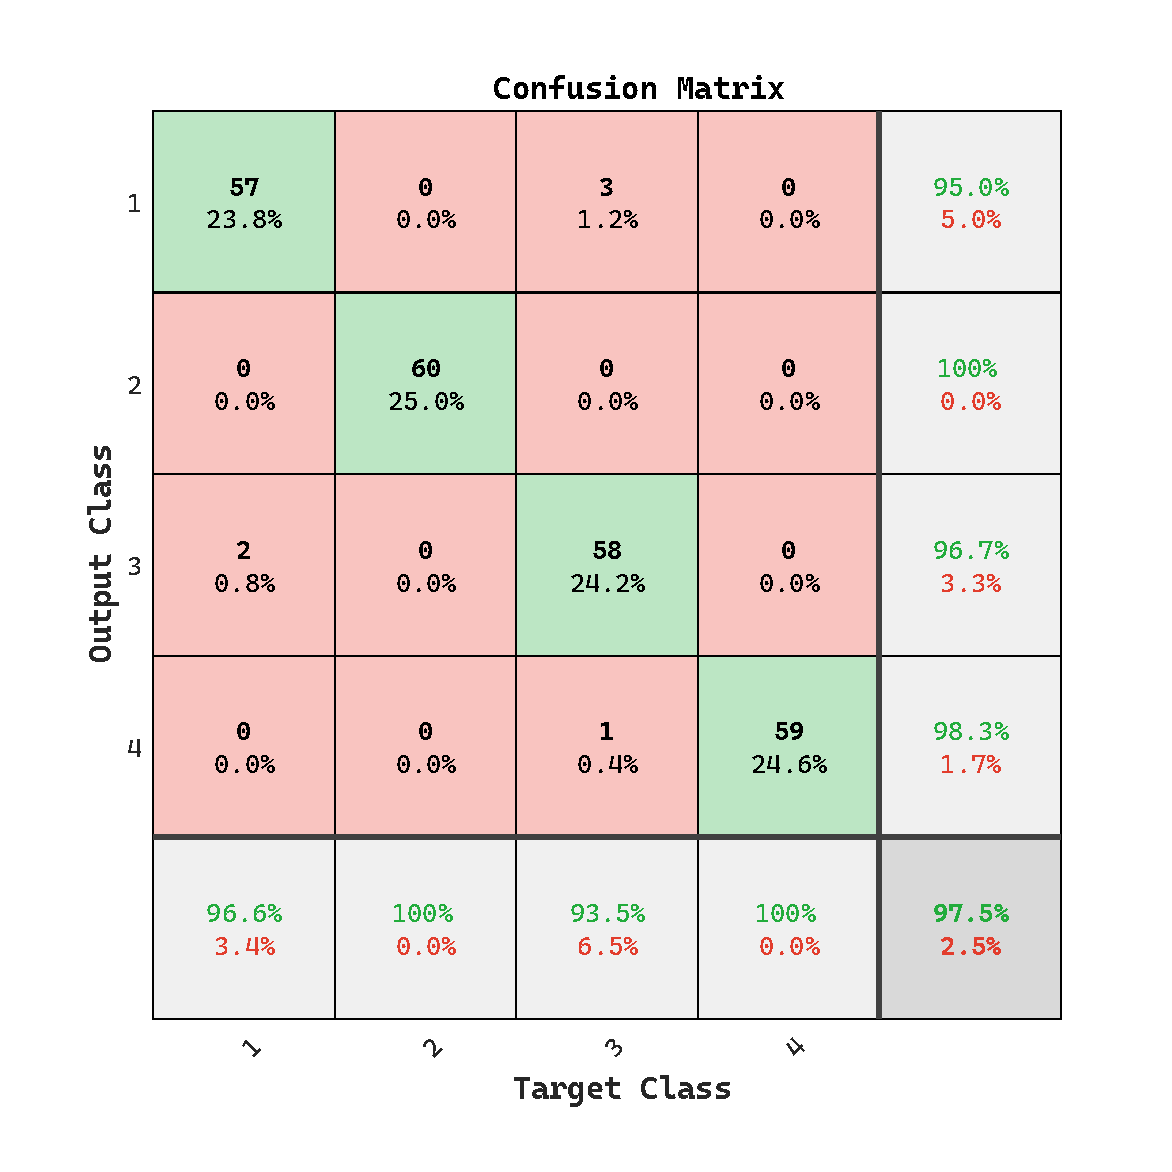
\includegraphics[width=0.49\textwidth]{addestramento-rete-neurale/two-liscio.pdf}
    \caption{Confusion matrix dell'allenamento con TL 2R senza preprocessing e con una semplice data augmentation}
    \label{fig:result-two-liscio}
\end{figure}

Per effettuare un allenamento 2R è sufficiente duplicare il codice di un TL facendo attenzione a usare la stessa rete.

\section{Image preprocessing}\label{image-preprocessing}

Un primo filtro di image preprocessing è modificare il contrasto dell'immagine, come noto il contrasto di una immagine influenza molto la vista umana, e dato che le \gls{cnn} sono molto simili al modello di connettività dei neuroni nel cervello umano è plausibile che modifiche al contrasto influenzano i risultati  ottenuti. Un semplice filtro per il contrasto si ottiene con:
\begin{lstlisting}
IM=imadjust(IM,[.2 .3 0; .6 .7 1],[]);    
\end{lstlisting}

In figura \cref{fig:result-contrast} sono presenti le confusion matrix dei risultati ottenuti con la modifica del contrasto.

\begin{figure}[H]
    \centering
    \begin{subfigure}{0.49\textwidth}
        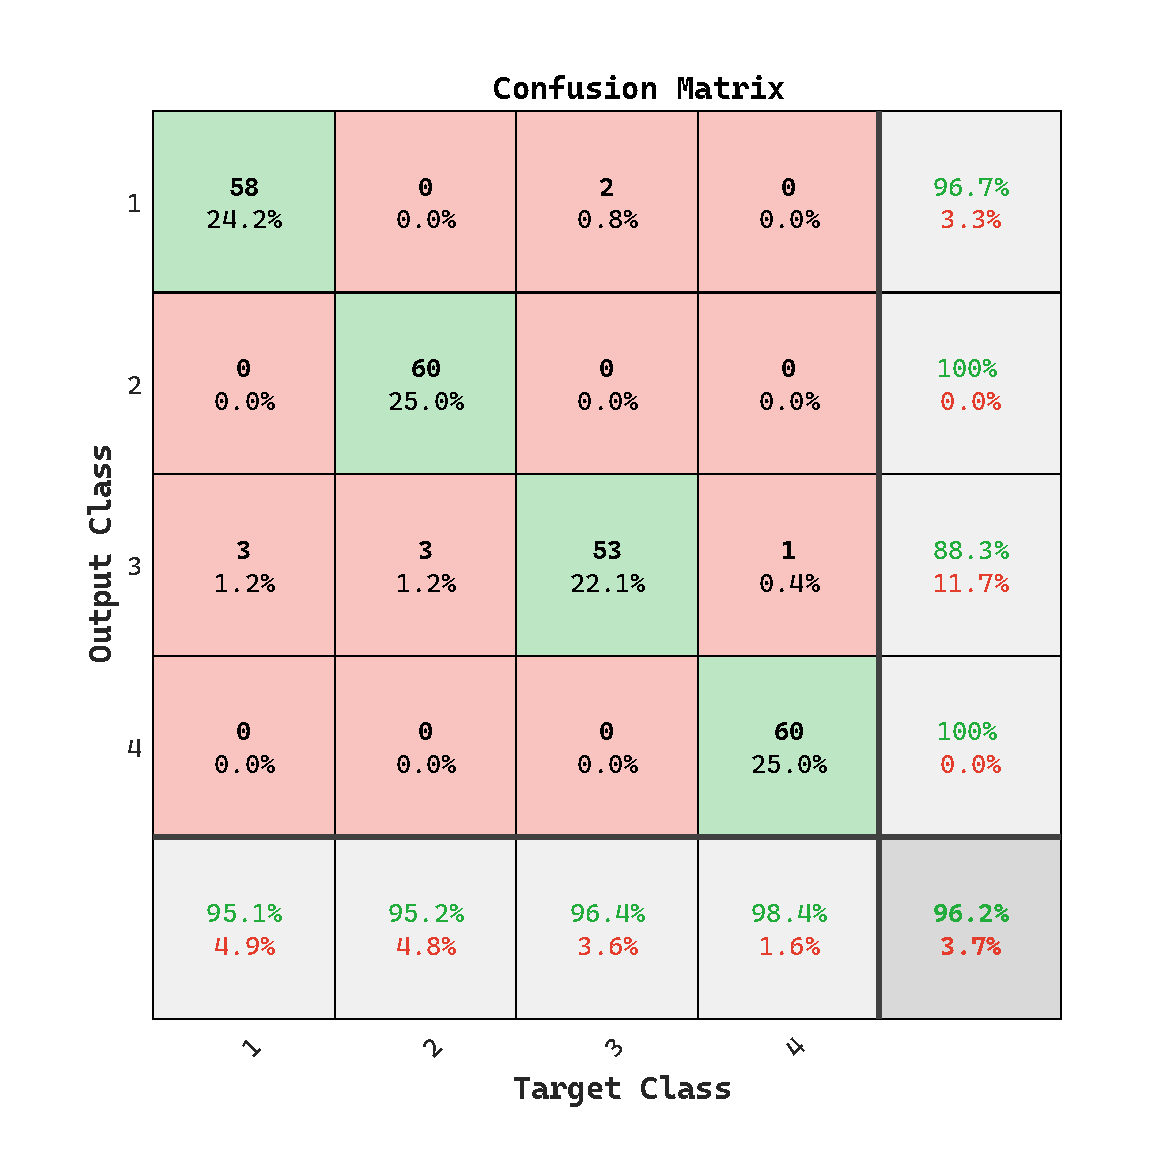
\includegraphics[width=\textwidth]{addestramento-rete-neurale/one-contrast.pdf}
        \caption{Allenamento 1R} 
    \end{subfigure}
    \begin{subfigure}{0.49\textwidth}
        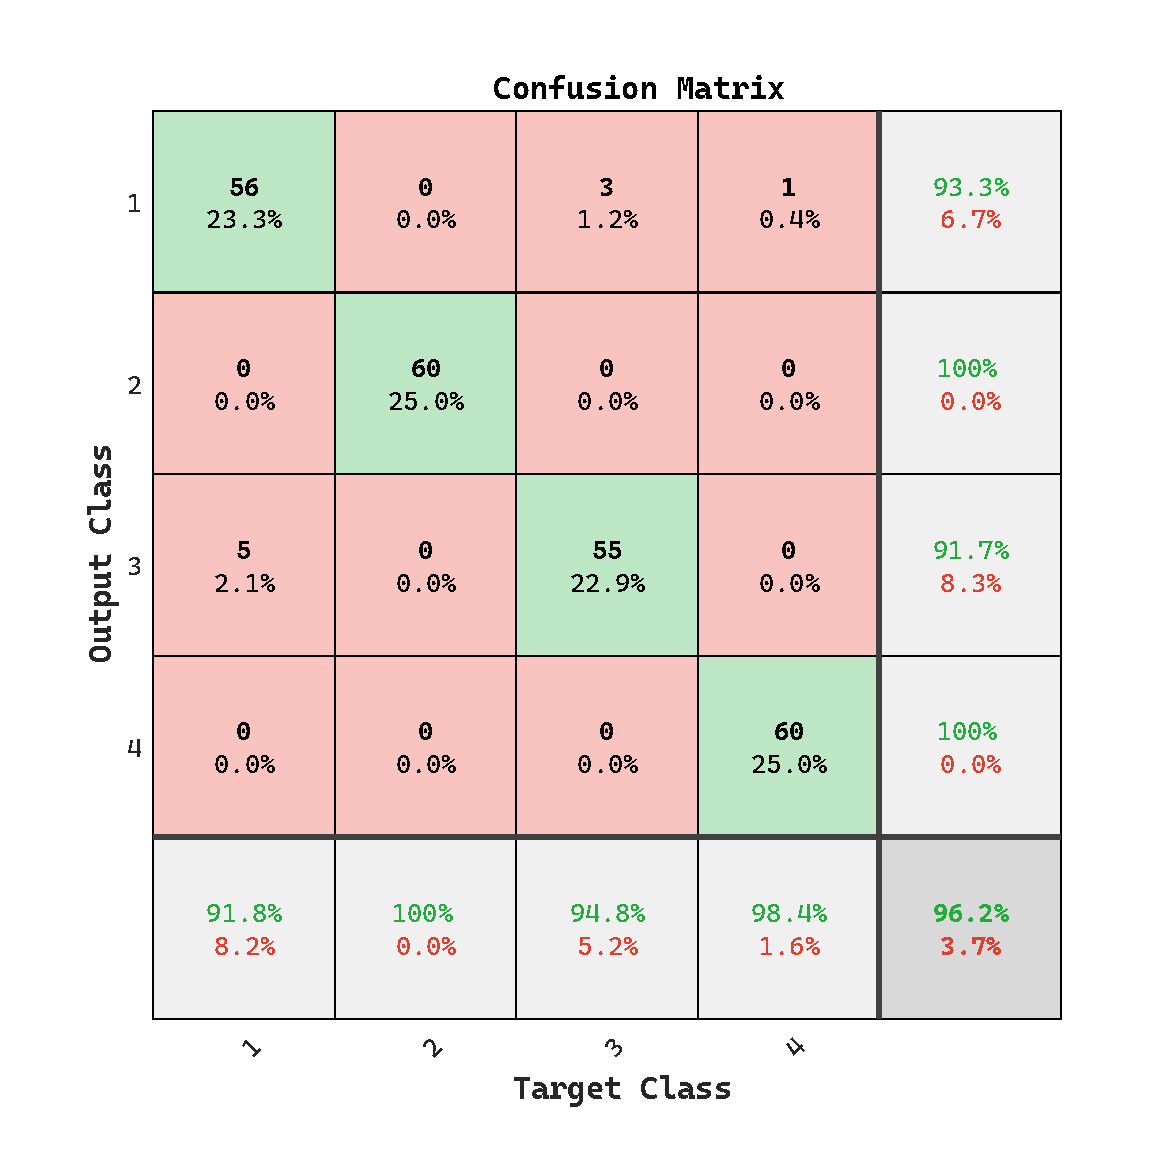
\includegraphics[width=\textwidth]{addestramento-rete-neurale/two-contrast.pdf}
        \caption{Allenamento 2R} 
    \end{subfigure}
    \caption{Confusion matrix dell'allenamento con TL 1R e 2R con correzzione contrasto hardcoded}
    \label{fig:result-contrast}
\end{figure}

Dato che nella preelaborazione precedente si usa un filtro hardcoded, lo step successivo è modificare il  contrasto in base alla media e alla derivazione standard dell'immagine (con \lstinline{n} un iperparametro che indica quanto modificare il contrasto). In \cref{fig:result-contrast-bis}  la confusion matrix con i risulati ottenuti con una correzione contrasto dinamica.
\begin{lstlisting}
n = 0.5;  
Idouble = im2double(IM); 
avg = mean2(Idouble);
sigma = std2(Idouble);
IM = imadjust(IM,[avg-n*sigma avg+n*sigma],[]);
\end{lstlisting}

\begin{figure}[H]
    \centering
    \begin{subfigure}{0.49\textwidth}
        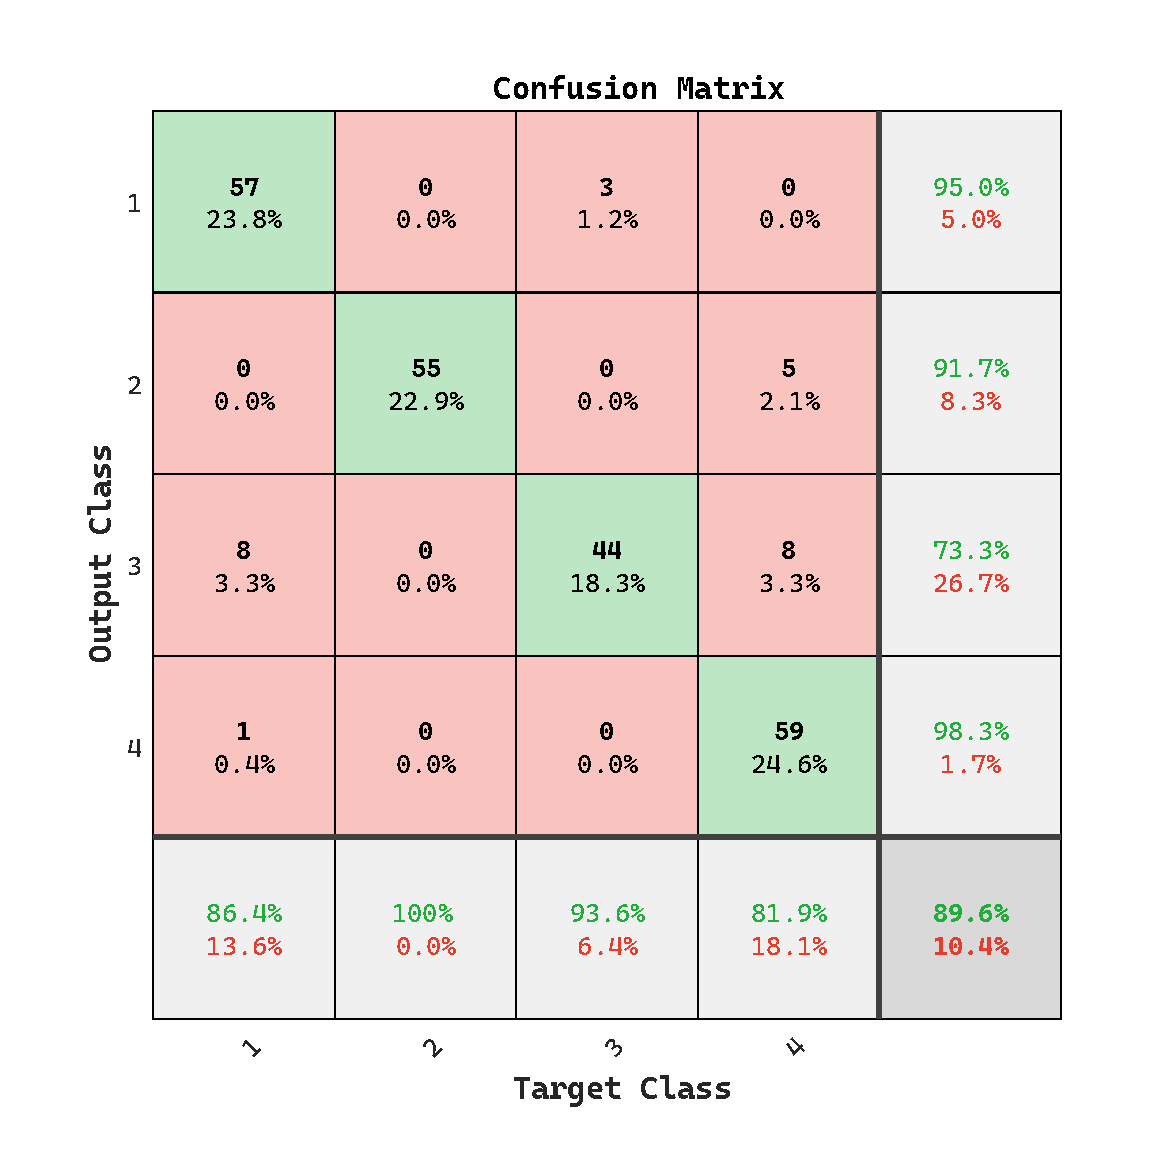
\includegraphics[width=\textwidth]{addestramento-rete-neurale/one-contrast-bis.pdf}
        \caption{Allenamento 1R} 
    \end{subfigure}
    \begin{subfigure}{0.49\textwidth}
        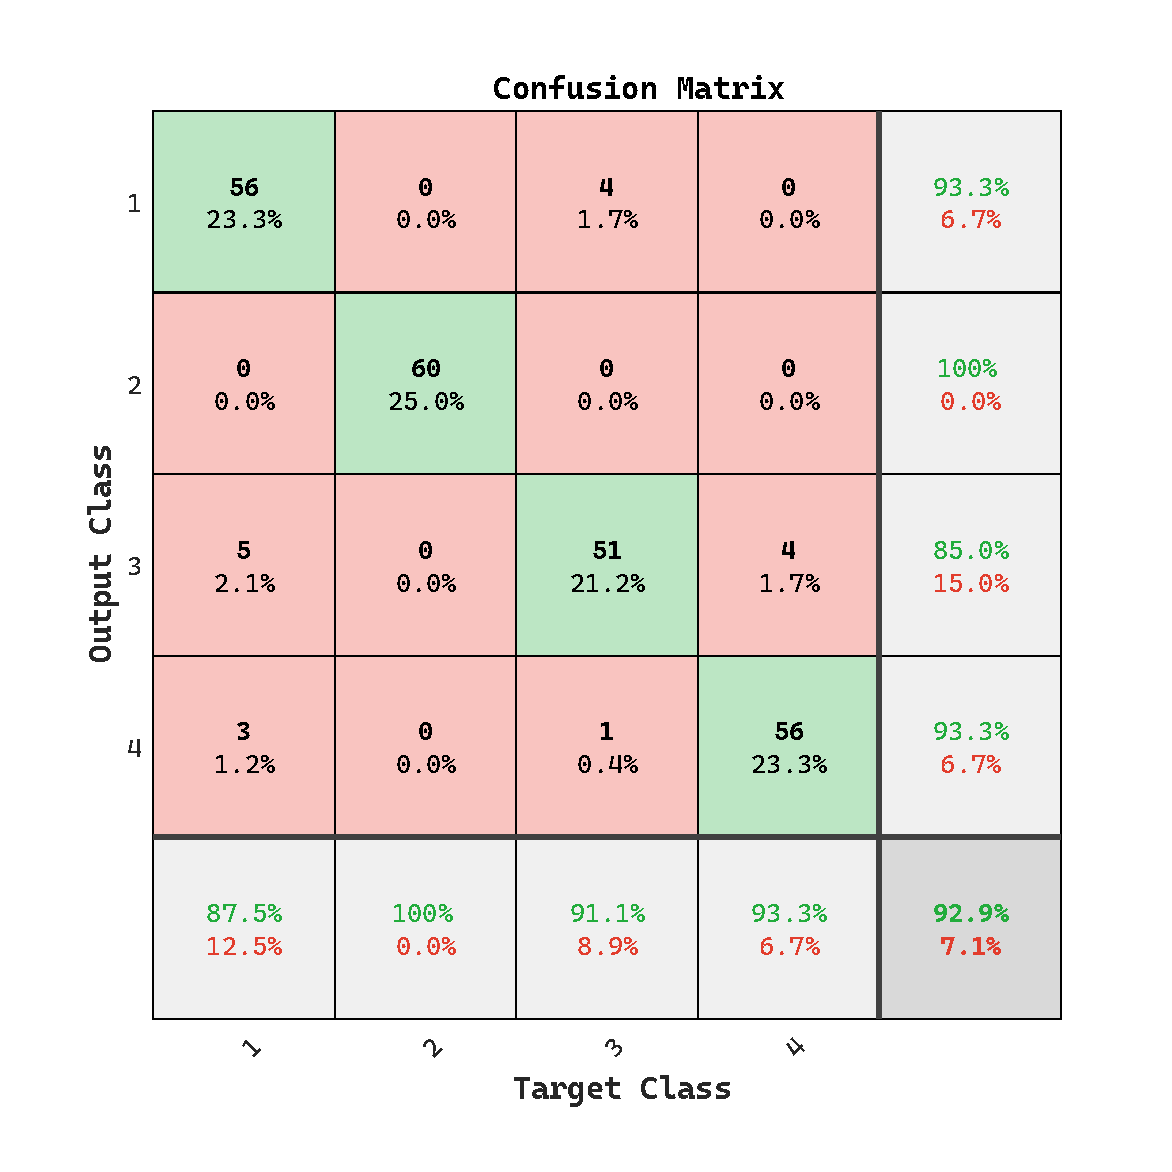
\includegraphics[width=\textwidth]{addestramento-rete-neurale/two-contrast-bis.pdf}
        \caption{Allenamento 2R} 
    \end{subfigure}
    \caption{Confusion matrix dell'allenamento con TL 1R e 2R con correzione contrasto dinamica}
    \label{fig:result-contrast-bis}
\end{figure}

Una versione più avanzata per l'elaborazione del contrasto è il CLAHE, il codice è descritto nel listato successivo e i risultati in \cref{fig:result-clahe}. 

\begin{lstlisting}
[X, MAP] = rgb2ind(IM, 65536);
RGB = ind2rgb(X,MAP);
LAB = rgb2lab(RGB);
L = LAB(:,:,1)/100;
L = adapthisteq(L,'NumTiles',[8 8],'ClipLimit',0.005);
LAB(:,:,1) = L*100;
IM = lab2rgb(LAB);
\end{lstlisting}

\begin{figure}[H]
    \centering
    \begin{subfigure}{0.49\textwidth}
        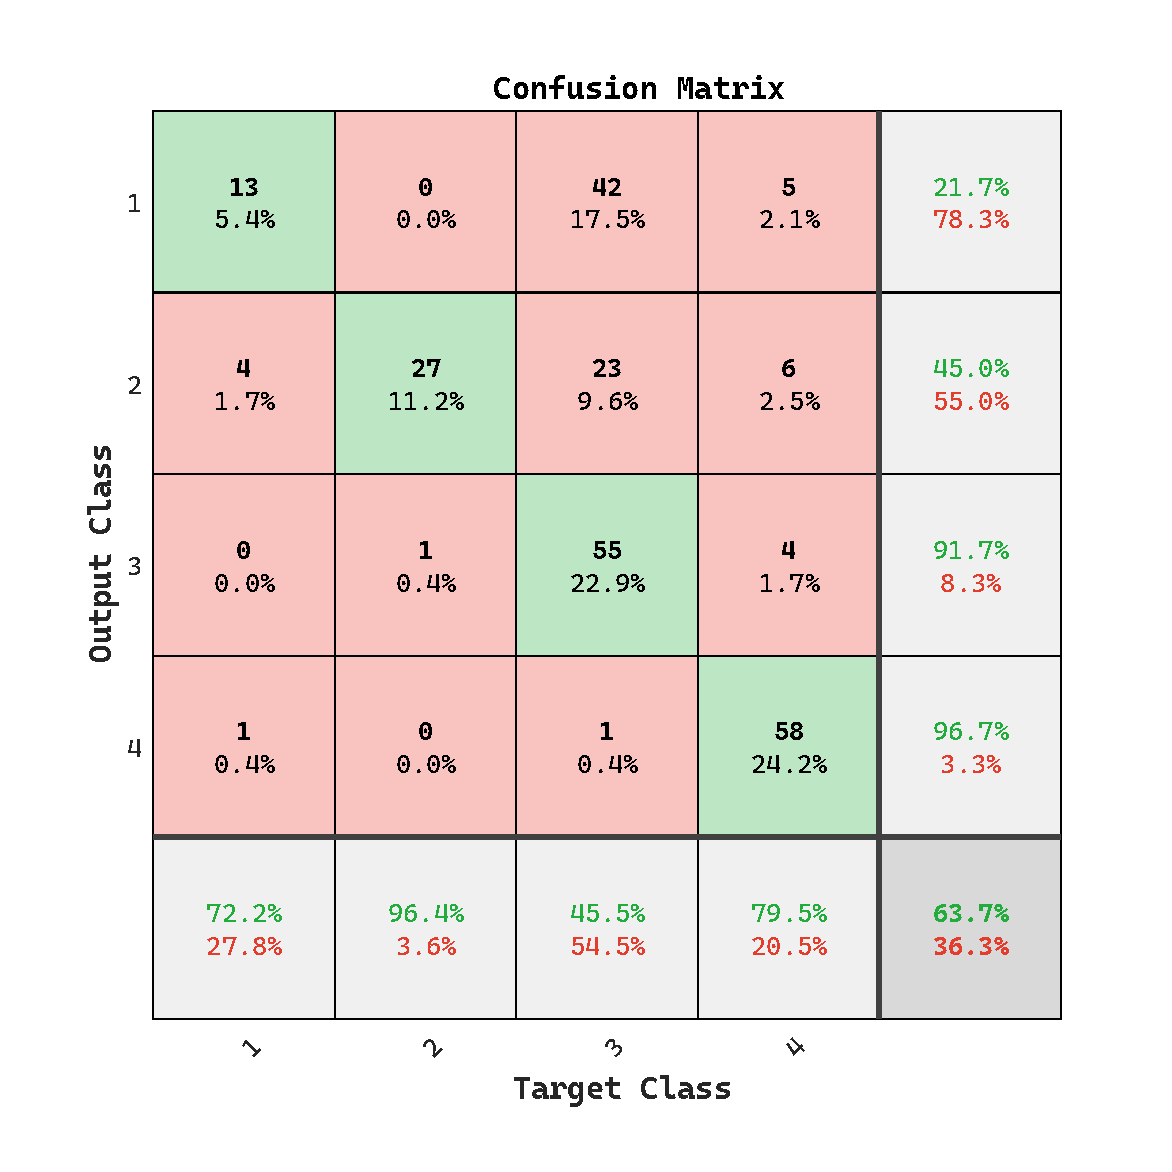
\includegraphics[width=\textwidth]{addestramento-rete-neurale/one-clahe.pdf}
        \caption{Allenamento 1R} 
    \end{subfigure}
    \caption{Confusion matrix dell'allenamento con  CLAHE}
    \label{fig:result-clahe}
\end{figure}

Per effettuare un miglioramento della Gamma (descritto in \cref{gamma}) dell'immagine e renderla più simile a quella dell'occhio umano si può usare il seguente codice, i risultati sono in \cref{fig:result-gamma}.

\begin{lstlisting}
hgamma = vision.GammaCorrector(2.0,'Correction','De-gamma');

IM= hgamma(IM);
\end{lstlisting}

\begin{figure}[H]
    \centering
    \begin{subfigure}{0.49\textwidth}
        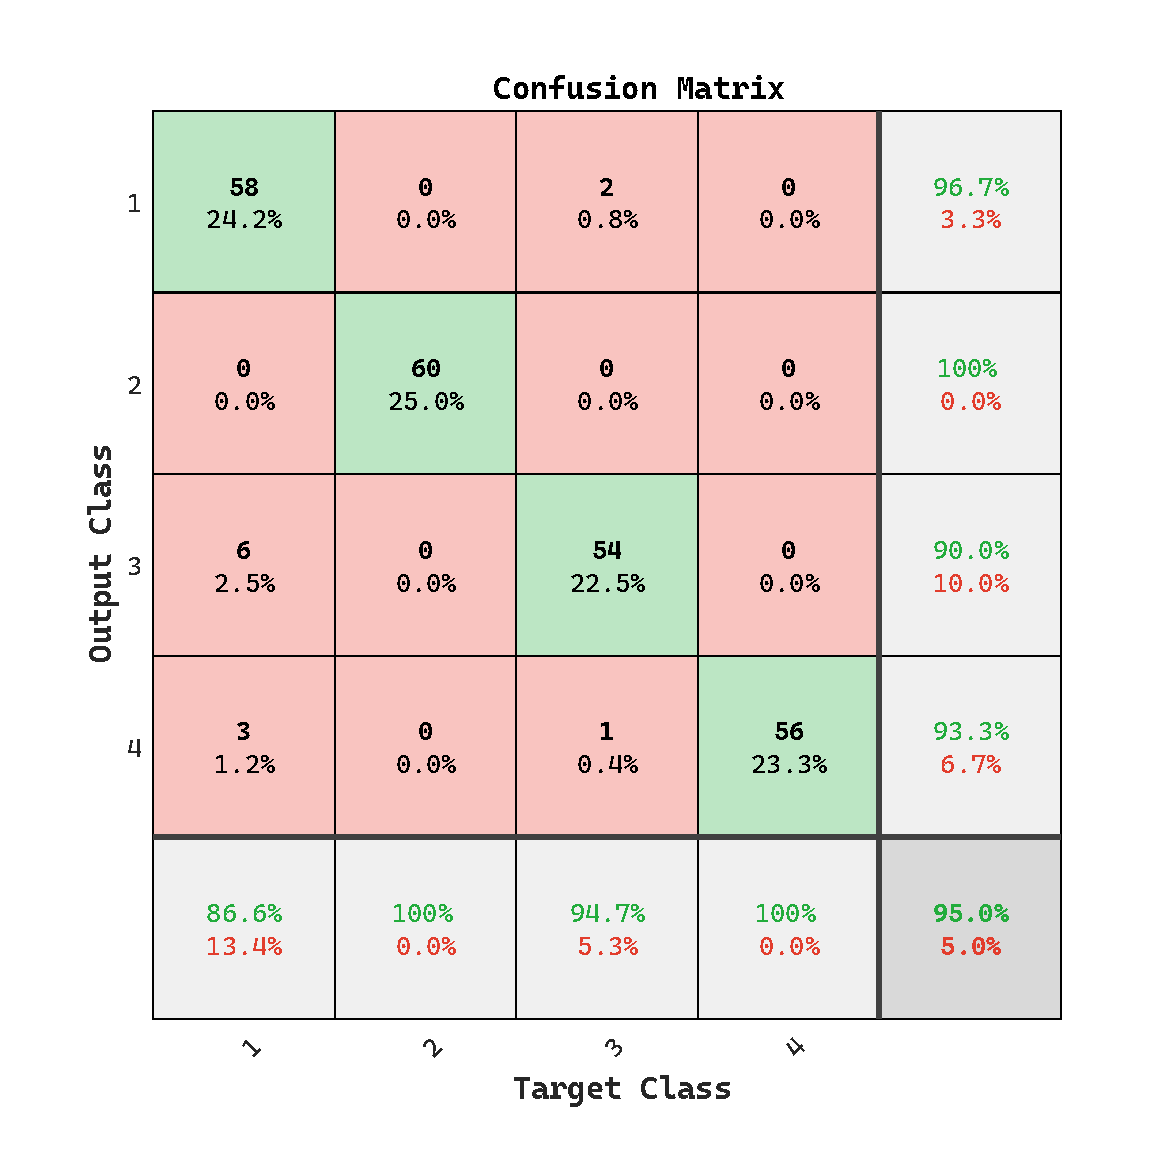
\includegraphics[width=\textwidth]{addestramento-rete-neurale/one-gamma.pdf}
        \caption{Allenamento senza CLAHE} 
    \end{subfigure}
    \begin{subfigure}{0.49\textwidth}
        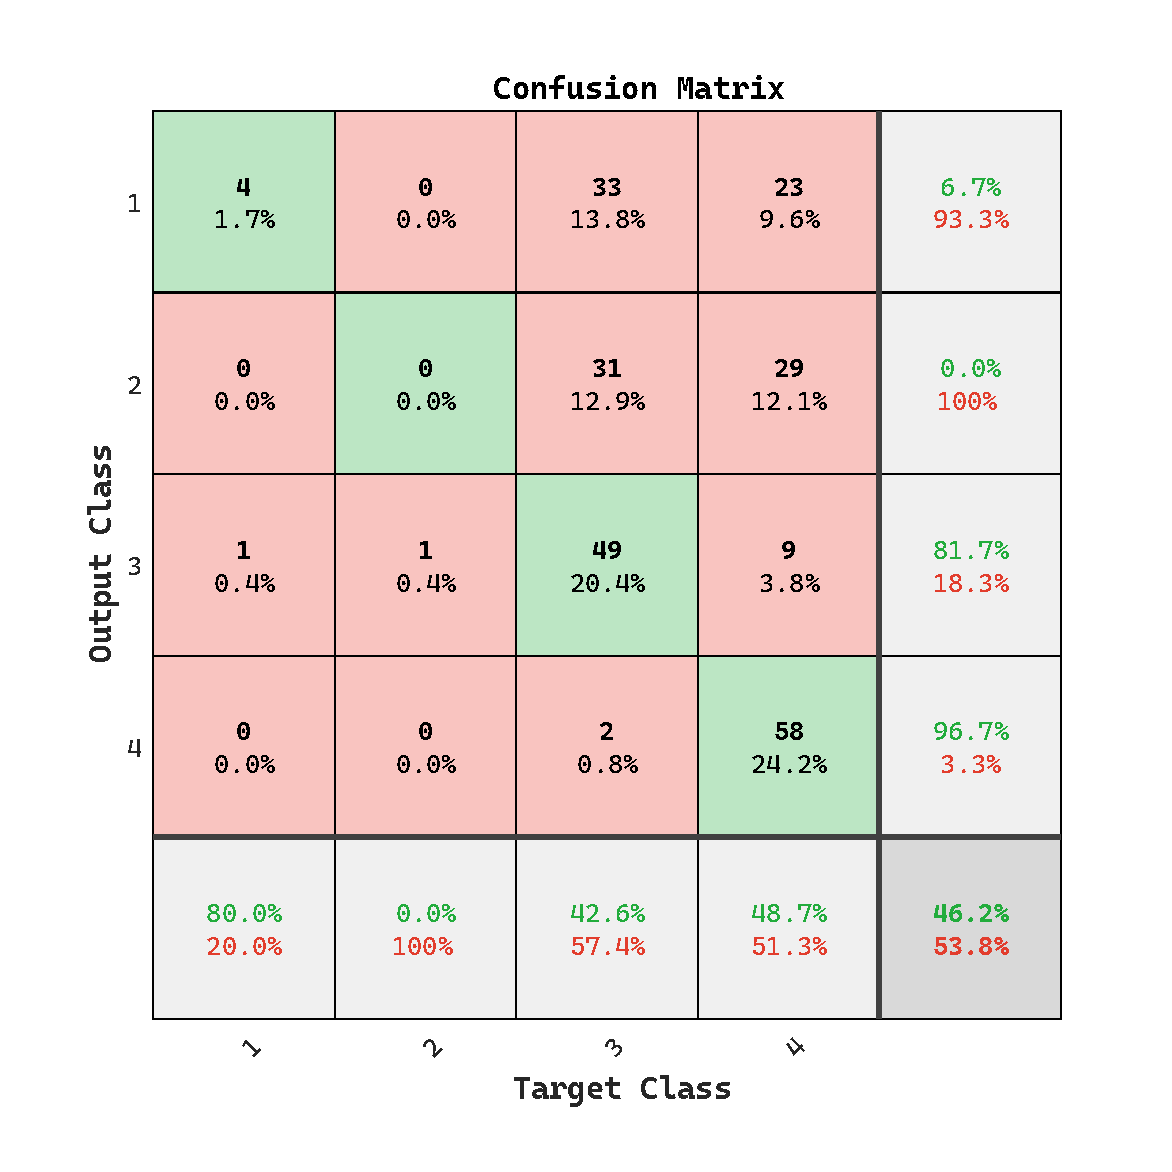
\includegraphics[width=\textwidth]{addestramento-rete-neurale/one-clahe-gamma.pdf}
        \caption{Allenamento con CLAHE} 
    \end{subfigure}
    \caption{Confusion matrix dell'allenamento con ottimizzazione gamma}
    \label{fig:result-gamma}
\end{figure}

Per aggiungere rumore artificiale all'immagine ed evitare che l'immagine si concentra su feature secondarie che potrebbero determinare basse prestazioni nei test set, i risultati sono in \cref{fig:result-noise}.

\begin{lstlisting}
IM = imnoise(IM,'salt & pepper',0.02);
\end{lstlisting}

\begin{figure}[H]
    \centering
    \begin{subfigure}{0.49\textwidth}
        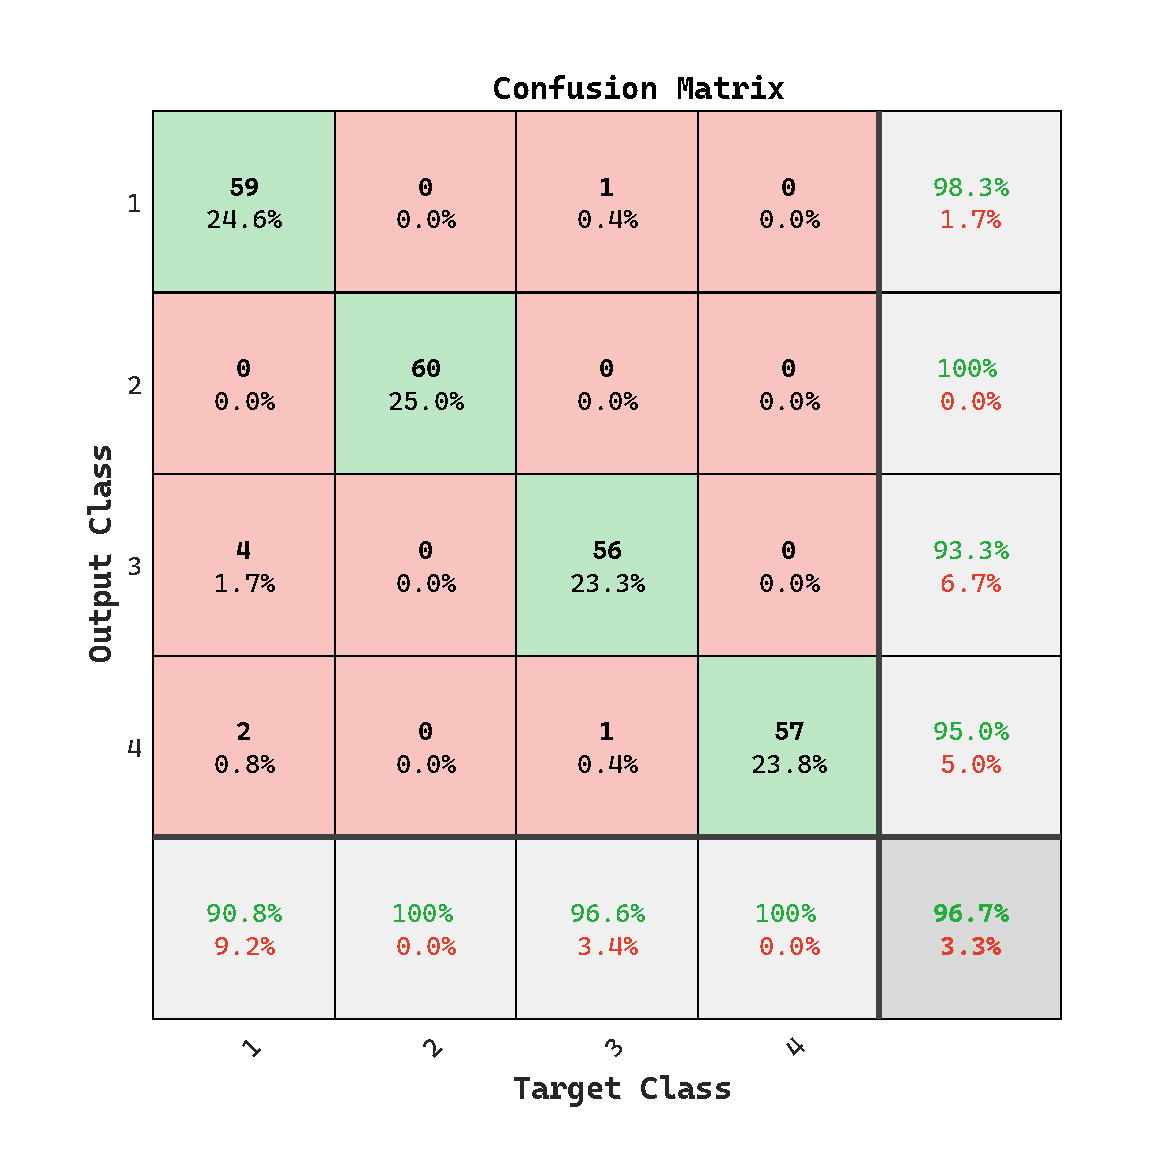
\includegraphics[width=\textwidth]{addestramento-rete-neurale/one-noise.pdf}
        \caption{Allenamento 1R} 
    \end{subfigure}
    \begin{subfigure}{0.49\textwidth}
        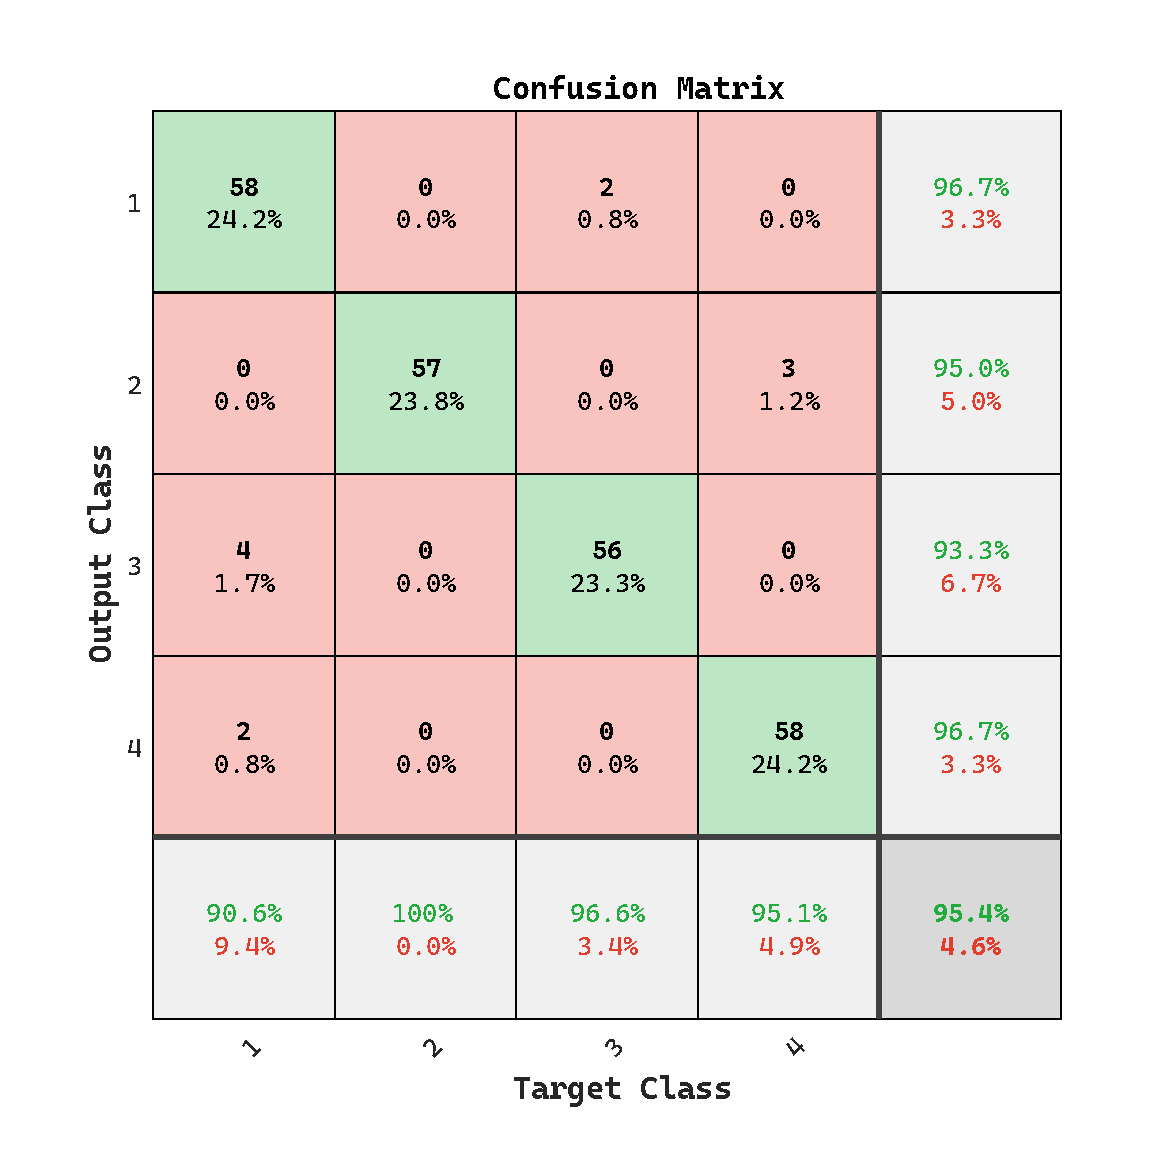
\includegraphics[width=\textwidth]{addestramento-rete-neurale/two-noise.pdf}
        \caption{Allenamento 2R} 
    \end{subfigure}
    \caption{Confusion matrix dell'allenamento con TL 1R e 2R con aggiunta di rumore artificiale}
    \label{fig:result-noise}
\end{figure}

\section{Data argumentation con DCT}\label{data-argumentation-con-dct}

Ci sono numerosi metodi per eseguire la DCT ed la relativa data augmentation, in particolare in \cref{discrete-cosine-transform-dct} sono illustrati due algoritmi. Il primo che per ogni frequenza la annulla con probabilità 0.5 e la seconda che la attenua con probabilità \(z\sim U\left(-\frac{1}{2}, \frac{1}{2}\right)\) \cite{nanni_dct_pca}. I risultati con DCT e Noise sono illustrati nelle confusion matrix della \cref{fig:result-dct-noise}.

\begin{figure}[H]
    \centering
    \begin{subfigure}{0.49\textwidth}
        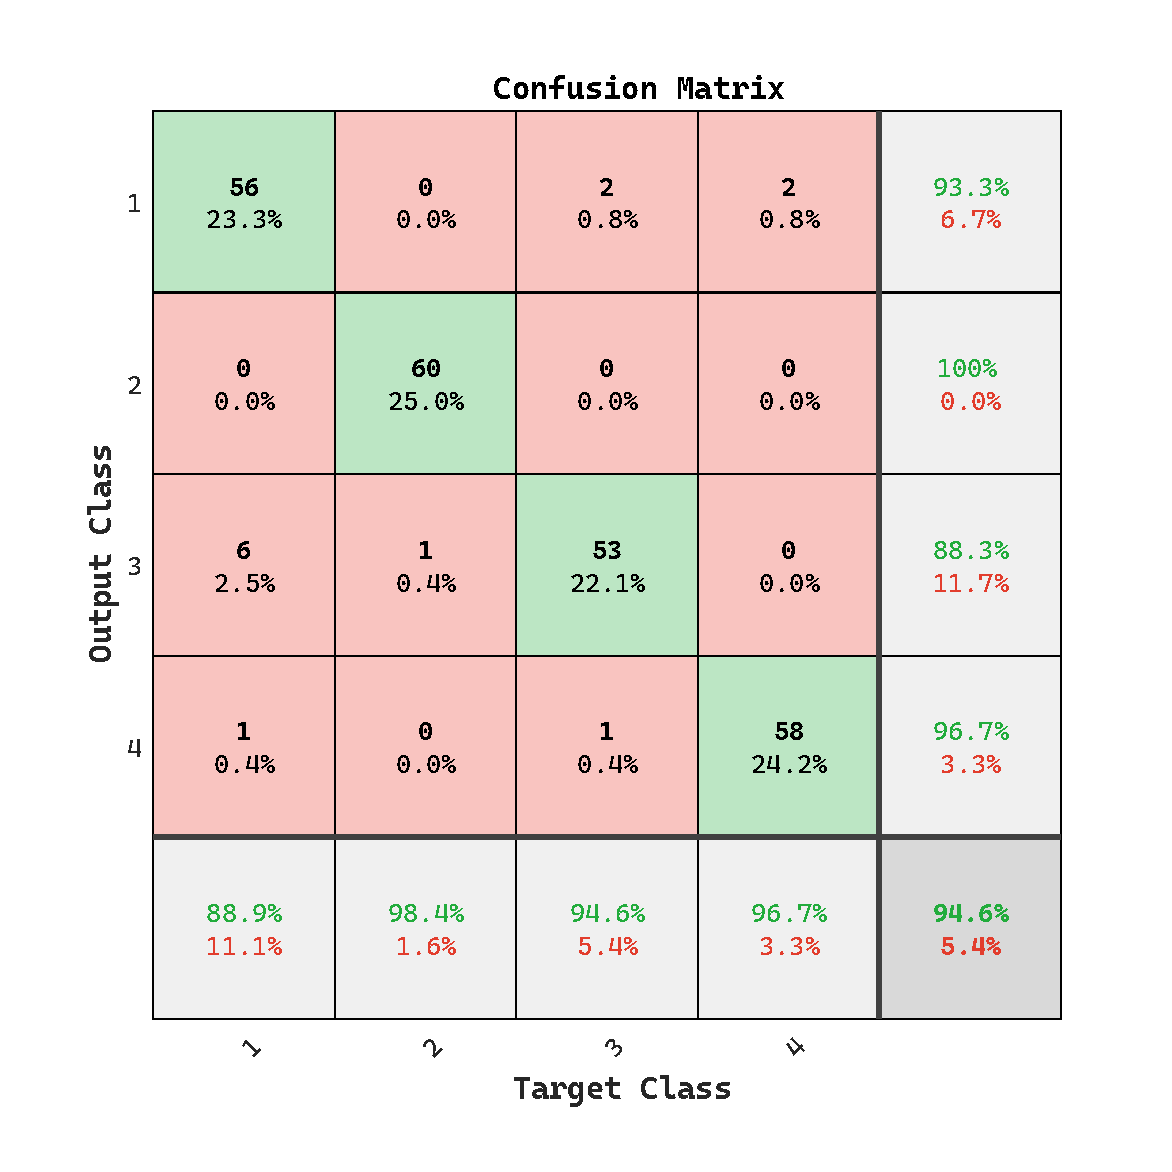
\includegraphics[width=\textwidth]{addestramento-rete-neurale/one-dct.pdf}
        \caption{Allenamento 1R} 
    \end{subfigure}
    \begin{subfigure}{0.49\textwidth}
        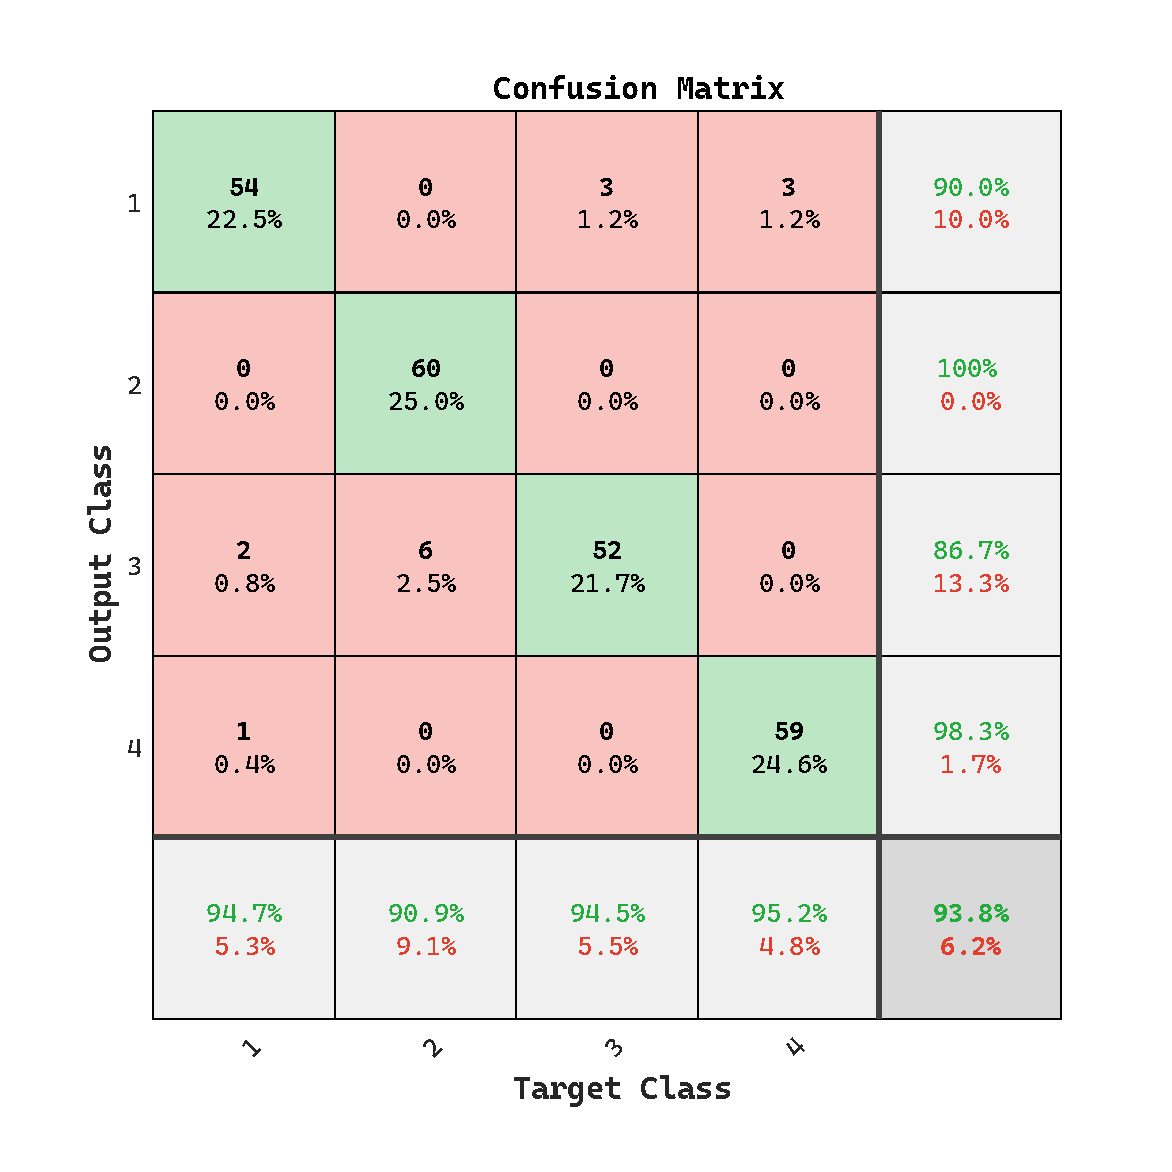
\includegraphics[width=\textwidth]{addestramento-rete-neurale/two-dct.pdf}
        \caption{Allenamento 2R} 
    \end{subfigure}
    \caption{Confusion matrix dell'allenamento con TL 1R e 2R con DCT e noise}
    \label{fig:result-dct-noise}
\end{figure}


\section{Risultati}\label{risultati}

In \cref{tab:specchio-single} c'è uno specchio riassuntivo dei vari risultati ottenuti in questa sperimentazione, riassumento le confusion matrix dei paragrafi precedenti.

\begin{table}[H]
    \centering
    \begin{tabular}{l|cc|cc}
                                     & \multicolumn{2}{c|}{1R}                                                   & \multicolumn{2}{c}{2R}                                                   \\
                                     & (1) & (2) & (1) & (2) \\ \midrule
    Semplice DA                      & 95.4\%                            & 100\%                                & 97.5\%                            & 100\%                                \\
    Filtro Contrasto Semplice        & 96.2\%                            & 100\%                                & 96.2\%                            & 100\%                                \\
    Filtro Contrasto con media e STD & 89.6\%                            & 91.7\%                               & 92.9\%                            & 100\%                                \\
    CLAHE                            & 63.7\%                            & 45.8\%                               &                                   &                                      \\
    Correzione Gamma                 & 95.0\%                            & 100\%                                &                                   &                                      \\
    Correzione Gamma e CLAHE         & 46.0\%                            & 0\%                                  &                                   &                                      \\
    Noise                            & 96.7\%                            & 100\%                                & 95.4\%                            & 95.0\%                               \\
    DCT e Noise                      & 94.6\%                            & 100\%                                & 93.8\%                            & 100\%                             
    \end{tabular}
    \caption{Specchio riassuntivo delle performance singole dei vari metodi analizzati, (1): Divisione corretta nelle 4 classi, (2): Riconoscimento dei frame Informative}
    \label{tab:specchio-single}
\end{table}


